\documentclass[12pt,a4paper]{article}

% Packages
\usepackage[margin=1.5in]{geometry}
\usepackage{graphicx}
\usepackage{float}
\usepackage{booktabs}
\usepackage{caption}
\usepackage{amsmath,amssymb}
\usepackage{siunitx}
\usepackage[hidelinks]{hyperref}
\usepackage{enumitem}
\usepackage{titlesec}
\usepackage[backend=biber,style=numeric-comp,sorting=none]{biblatex}
\usepackage[table]{xcolor}
\usepackage{algorithm}
\usepackage{algpseudocode}
\usepackage{indentfirst}    
\addbibresource{references.bib}
      
\setlength{\parindent}{1.5em}     
\setlength{\parskip}{0.8\baselineskip} % gap between subsequent paragraphs


% spacing: before section = 0.8 line, after section = 0 (no gap)
\titlespacing*{\section}{0pt}{0.8\baselineskip}{0pt}
\titlespacing*{\subsection}{0pt}{0.6\baselineskip}{0pt}

% Formatting
\titleformat{\section}{\Large\bfseries}{\thesection}{0.8em}{\MakeUppercase}
\titleformat{\subsection}{\normalsize\bfseries}{\thesubsection}{0.6em}{\MakeUppercase}
\newlist{steps}{enumerate}{1}
\setlist[steps,1]{label={[{\arabic*}]}, leftmargin=*, itemsep=0.3em}
\captionsetup{font=small, labelfont=bf}

% Metadata
\title{\centering {\textbf{CNN-Based Investment Strategies with Integrated Technical and Macroeconomic  Representations}}}
\author{Vall James P. Luceres \\
CMSC 199.1: Research in Computer Science I \\
Division of Natural Sciences and Mathematics \\
University of the Philippines Tacloban College \\
Tacloban City, Philippines \\
vpluceres@up.edu.ph}
\date{\today}

\begin{document}
\maketitle
\thispagestyle{empty}     
\pagenumbering{gobble}    

\newpage
\begin{abstract}
Market behavior is shaped not only by price movements but also by macroeconomic forces that influence price stability. Current quantitative trading systems that are built on convolutional neural networks (CNNs) typically represent market dynamics using technical indicator images. However, these models often ignore macroeconomic indicators that significantly influence asset returns. This study will focus on integrating technical indicator image representations with macroeconomic indicators to enhance decision quality in data driven investment strategies by improving the classification accuracy of the assigned trading label (Buy, Hold, or Sell). Using a 20-day window size, the study combines technical indicators and macroeconomic informed representations to generate images for each trading day. In order to evaluate its performance, quantitative trading simulations were conducted on various Philippine stocks across different categories such as blue-chip, penny stocks, and cryptocurrency. Initial findings reveal that incorporating macroeconomic representation increases prediction accuracy and provides enhanced trading performance compared to CNN-based models that rely solely on technical indicator images. These results indicate that such application allows models to better capture both technical indicators and macroeconomic-informed representations, therefore producing more consistent outcomes across diverse trading environments. 
\newline

\textit{Keywords}: Deep-learning; image classification; trading indicators; macroeconomic-informed representations; quantitative trading strategies
\end{abstract}
\newpage
\tableofcontents
\newpage
\clearpage
\setcounter{page}{1}      % start counting here
\pagenumbering{arabic}    % turn ON 1,2,3...

\section{Introduction}

Market behavior is shaped not only by price movements but also by the broader economic context that affects risk, liquidity, and investor behavior. Over the past decade, computer vision-based models have become a popular tool that convert price data into images and train Convolutional Neural Networks (CNN) to generate \textit{Buy/Hold/Sell} decisions \cite{cohen2020trading,sezer2018algorithmic,gudelek2017deep}. These are effective in capturing local patterns of time and price. However they usually treat the macroeconomic context separately, which has a clear contribution to changing market prices \cite{wang2019aggregating,ma2022macroeconomic,chauhan2025exploring}.

This study aims to improve existing image-based representations by merging technical and macroeconomic indicators into a unified image representation so that it can be processed by our proposed CNN model. 
The model takes into account strict time adaptation, uniform normalization, and careful encoding to preserve the relationship between local patterns and market context \cite{sezer2018algorithmic,maratkhan2021deep}. 
The framework is applied to selected Philippine blue-chip, penny stocks, and cryptocurrency, where the impact of incorporating macroeconomic indicators on prediction accuracy and performance metrics is measured.

\subsection{Background of the Study}
	\subsubsection*{Quantitative Trading using Image Classification}
	Quantitative trading is a system that automates trades that are conducted using models and technical indicators as tools \cite{ta2018prediction}. It can be represented in images that are in a grid of indicators and time windows, to allow spatial filters to uncover patterns that match price movement \cite{cohen2020trading,sezer2018algorithmic}. Representations such as candlesticks, bar charts, and technical indicators as images can improve trend classification and transaction signals \cite{gudelek2017deep,chen2020encoding,liu2023automated}. Transforming financial time series into visual representations enables machine learning algorithms to efficiently recover complex trading signals \cite{cohen2020trading}, with candlestick image data consistently outperforming traditional numeric approaches \cite{liu2023automated}. 


	\subsubsection*{CNN based Technical Indicator Clustering (CNN--TIC)}
	Convolutional neural networks are structured to learn spatial patterns from grid formatted data, which makes them well suited for technical indicators that are arranged as two dimensional images \cite{al2017understanding,lecun1995learning}. Early image based trading studies demonstrated that converting technical indicator into fixed size grayscale images allows a CNN to detect local price and momentum patterns more effectively than traditional numeric inputs \cite{sezer2018algorithmic}. This established image representation as a practical way to capture short term market patterns.
	
	Later work organized indicators into clustered channels, forming what is now known as the CNN--TIC model \cite{maratkhan2021deep}. This formulation groups related features such as trend, momentum, and volatility indicators so the CNN can learn joint relationships across clusters rather than processing each indicator independently. The structured layout enables the model to extract more coherent visual patterns from technical indicators, making CNN--TIC a reliable baseline for quantitative image based trading systems.
	

	\subsubsection*{Multimodal Approach}
	In deep learning, multimodal processing refers to the integration of data from different types to increase the learning efficiency and performance of algorithms on a specific task \cite{dimitri2022short}. This approach is advantageous because each modality responds to different characteristics and provides complementary information that is not fully captured by a single form of data. For example, visual data can support and validate the content of spoken language, while textual data can explain the content of visual cues. In the context of financial market, the technical picture from OHLCV depicts local patterns over time and price, while textual policy statements, earnings reports, and sentiment measures on social media provide a more slowly evolving context of market environment and risk \cite{farimani2024adaptive,karadacs2025multimodal}.

	These representations provide a broader range of signals that can help to understand the change and risk of the market environment \cite{zhang2020multimodal}. Fusion can be viewed as the combination of different modalities into a single meaning space, so that the learned patterns are richer, more robust to noise, and more appropriate to different market conditions. Additionally, it can also be presented in a form that is well-suited for learning that can improve classification and prediction compared to relying on a single approach \cite{gallo2018image}. 

	\subsubsection*{Macroeconomic Representation}
	Macroeconomic representations are economic signals such as interest rates, inflation, exchange rates, market volatility, and foreign investment, that reflect the state of the market environment at a given time \cite{artantacs2020selected}. This is relevant because literature shows that macroeconomic attention and policy uncertainty are significantly linked to expected short and long term earnings and sector dynamics \cite{ma2022macroeconomic}. In this view, the macro series becomes the “context” that moves slowly and shapes the course of market and liquidity, while technical indicators from OHLCV represent the faster, more localized patterns. It is important to describe these signals in a consistent form and scale that can be related to the technical representation \cite{wang2019aggregating}.

	In this study, the model is trained on a macroeconomic representation combined with technical indicators which will potentially increase the accuracy for market prediction models and have a good trading performance. Selected key indicators are interest rates, purchasing power of the peso, Reverse Repurchase (RRP), gold, and crude oil which are subjected to a uniform normalization to achieve a uniform scale, and are adapted to the trading calendar to maintain meaningful correlations with local patterns. In this format, the contribution of the macroeconomic context will not just be a substitute but as a complement to improving the classification and prediction during different market conditions.



\section{Related Works}
The evolution of financial market prediction using computer vision is slowly becoming a popular tool used in trading. Previous studies surrounding market prediction can be categorized into three categories. To start, we have numerical models that are solely trained on technical indicators. Another approach is by using computer vision, which analyzes chart-based or image representations of price series. Lastly, multimodal fusion models that cover signals such as prices, technical indicators, and macroeconomic variables to improve prediction performance.

Chakole et al.\ \cite{chakole2021convolutional} introduced a Deep Trend Following (DTF) strategy that uses CNN prediction with market trend signals. The approach focuses on generating trading decisions based on the current and predicted future price of stocks. Results showed that their model provided a much better performance than traditional buy and hold models. Similar to this method, Saud et al.\ \cite{saud2024technical} used technical indicators such as MACD, DMI, and KST with LSTM models and GRU networks that can be used to develop intelligent strategies to predict stock trading signals. Their study showed that the MACD-based approach was the safest and most effective approach among other models. These results reinforce the role of technical indicators as a strong foundation for quantitative trading models.

Computer vision offers another effective approach in predicting the market price. Unlike the traditional numerical methods, computer vision trading focuses on analyzing visual representations such as candlesticks and bar charts. Cohen et al.\ \cite{cohen2020trading} pioneered this approach by transforming time-series analysis into image classification. This motivation came from financial traders that typically execute trades while observing charts. Liu et al.\ \cite{liu2023automated} further validated this method, demonstrating that models using candlestick image data outperformed those using numeric data.

The effectiveness of translating financial data into images is strongly demonstrated by a progression of studies from Sezer \cite{sezer2018algorithmic}. Building on earlier work that converted indicators into images (CNN-TA) and used bar-chart images (CNN-BI), Maratkhan et al.\ \cite{maratkhan2021deep} presented a highly optimized pipeline. Their architectures (CNN--TIC, EO--CNN--TIC, ResNet--TA) clustered technical indicators into multi-channel images and used an optimized trading layer to achieve remarkable results: ``Buy/Sell'' recall scores up to $0.94/0.96$ and average annual returns on DOW-30 up to $36.70\%$, substantially outperforming buy-and-hold and their own reproduced baselines. In addition, Wu \cite{wu2021empowering} specifically highlighted that computer vision techniques can address technical analysis objectives like predicting bullish/bearish trends. Then in 2019, Chen et al.\ \cite{chen2020encoding} developed approaches to automatically recognize candlestick patterns with over $80\%$ accuracy using convolutional neural networks, providing strong evidence for the effectiveness of visual representation in trading.

Studies on financial market forecasting also utilized multimodal fusion frameworks to enhance prediction accuracy by integrating different data sources. Wang et al.\ \cite{wang2019aggregating} pioneered a model-independent framework that successfully incorporated trading volume, intraday return series, and investors’ social media emotions to forecast market trends. This study demonstrates that combining multiple information sources significantly outperforms single-method approaches in financial market prediction. Ma et al.\ \cite{ma2022macroeconomic} proved that macroeconomic attention indices (MAI) can predict stock market returns by components that are extracted using partial least squares (PLS) and the LASSO method. Chauhan et al.\ \cite{chauhan2025exploring} had a similar study that used an ARDL model to reveal how macroeconomic indicators like Foreign Institutional Investment (FII) and Economic Policy Uncertainty (EPU) influence stock returns over both short and long terms.

Finally, researchers have fused textual and numerical data. Mo et al.\ \cite{mo2024mof} proposed a system that addresses key limitations in traditional stock prediction models by integrating policy and stock review texts with price data. The mechanism uses MacBERT to generate feature vectors and combine them with stock price data to be processed on a neural network. Similarly, Rahul Modak et al.\ \cite{Modak2023MarketSA} developed a multimodal transformer architecture that integrates earnings call transcripts, social media content, and technical market indicators, achieving $87.2\%$ sentiment classification accuracy compared to $78.4\%$ for unimodal baselines.


\section{Statement of the Problem}
\begin{figure}[H]
    \centering
    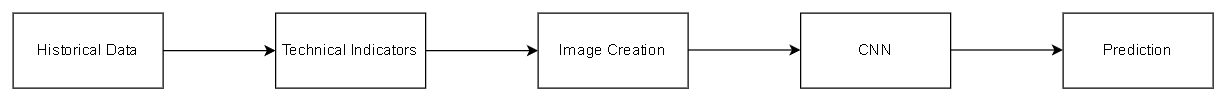
\includegraphics[width=0.8\textwidth]{figures/CNN-TIC.png}
    \caption{Computer-vision trading using technical indicators}
    \label{Figure 1: Computer-vision trading using technical indicators}
\end{figure}

Figure~\ref{Figure 1: Computer-vision trading using technical indicators}  illustrates a typical single mode workflow where historical price data are transformed into technical indicators, arranged as two dimensional images, and passed through a CNN to generate trading signals \cite{sezer2018algorithmic,gudelek2017deep}. This setup is effective in capturing local price-time patterns because convolutional filters can highlight short term structures on the image \cite{cohen2020trading}. However, the representation is restricted to indicators derived from OHLCV and does not explicitly incorporate macroeconomic information that shapes market risk, liquidity, and trend formation.

As a result, current CNN based image models provide an incomplete view of the market environment. Broader conditions such as changes in interest rates, inflation, or policy related uncertainty are not encoded in the same space as the technical picture, even if they have a documented effect on asset returns \cite{wang2019aggregating,ma2022macroeconomic,chauhan2025exploring}. In simple terms, existing CNN trading systems operate only on technical indicator images, and there is no unified image representation where technical signals and macroeconomic indicators are jointly organized, aligned, and scaled. This gap is the main problem that the study aims to address.


\section{Objectives of the Study}
\subsection{This study aims to}

\noindent Develop and evaluate an enhanced CNN-based trading model that integrates both technical and macroeconomic indicators to improve financial market trend prediction accuracy.
\subsection{The specific objectives of this study are as follows:}
\begin{steps}
  \item To enhance the CNN--TIC framework by expanding its technical indicator image matrix to include macroeconomic variables, forming a unified visual representation.
  \item To compare model performance using metrics such as accuracy, F1-score, and annualized return, to determine whether the inclusion of macroeconomic indicators leads to significant improvements.
  \item To evaluate performance on different stock categories in the PSE market and cryptocurrency.
  \item To evaluate feature importance and model behavior, interpret how macroeconomic information contributes to CNN decision-making in the context of financial trend prediction.
\end{steps}
\section{Scope and Limitation}
Previous studies on quantitative trading involve only CNNs that are solely trained on technical indicators
as image representations. In such settings, the absence of macroeconomic information may limit the robustness and accuracy of the resulting models. Thus, this study aims to develop and evaluate a CNN-based trading framework that integrates both technical and macroeconomic indicators into a
single image representation for market trend prediction.

The model will be tested on different stocks of the Philippine Stock Exchange (PSE) market, and will further include cryptocurrency data. The dataset will include historical daily price data, trading volumes, and selected
macroeconomic indicators such as reverse repurchase (RRP), purchasing power of peso, inflation rate, gold, and crude oil. Meanwhile, the technical indicators that will be used are relative strength index
(RSI), Williams \%R, simple moving average (SMA), exponential moving average (EMA), weighted moving average
(WMA), Hull moving average (HMA), triple exponential moving average (TEMA), commodity channel index (CCI),
Chande momentum oscillator (CMO), moving average convergence and divergence (MACD), percentage price
oscillator (PPO), rate of change (ROC), Chaikin money flow indicator (CMFI), directional movement indicator
(DMI), and parabolic SAR (PSI).

Although quantitative trading is focused on financial market prediction, this study will only focus on stock data
from the Philippine market, which may limit its applicability to other stock markets with different economic conditions. Additionally, trading simulations use a 50 pesos fixed commission per trade and ignores market slippage. Nonetheless, this study aims to develop a structured framework to identify how macroeconomically informed visual representations can enhance CNN-based trading performance across various
market conditions.

\section{Significance of the Study}
With the growing interest in applying computer vision for market trend prediction, the need to show how we can incorporate both technical and macroeconomic indicators into a single image representation becomes even more important. Unlike traditional CNN models that solely rely on technical indicators, the proposed CNN framework aims to improve predictive accuracy and financial returns across different market conditions that are driven by macroeconomic factors.

The research will contribute to developing more adaptive quantitative trading system that supports data-driven decision-making for traders and financial institutions. Academically, it extends computer vision applications in finance and provides a reproducible foundation for future studies on financial forecasting.

\section{Proposed Framework}
\begin{figure}[H]
    \centering
    
\includegraphics[width=0.8\textwidth]{figures/Proposed Framework.png}
    \caption{Proposed Framework}
    \label{Figure 3: Proposed Framework}
\end{figure}

This framework is based on two separate but related branches: the technical indicator branch from OHLCV-based indicators and the macroeconomic indicator branch that describes the market environment. The main goal is to combine the local pattern from the technical indicator and the macroeconomic context which will yield a higher representation. At the system level, the branches are organized, scaled and aligned on a common trading-day grid before being fused into a combined image representation.

After fusion, the merged image is passed to the CNN which acts as a spatial correlation extractor and provides an initial Buy/Hold/Sell prediction. Finally, the validity of the judgments is evaluated through partitioning and backtesting to see the performance under different market conditions.

In summary, Figure~\ref{Figure 3: Proposed Framework} illustrates the flow from data gathering, parallel technical and macro processing, fusion to CNN, and model evaluation. Each step will be explained in detail in the Methodology Section to clearly demonstrate the exact formulations, parameter choices, and evaluation criteria.

\section{Methodology}
\label{sec:methodology}

Figure~\ref{Figure 3: Proposed Framework} outlines the five stages of our methodology: \emph{Data Gathering}, \emph{Data Processing}, \emph{Image Creation}, \emph{Model Training}, and \emph{Model Evaluation}. The flow is centered on building an image representation of the combined technical and macroeconomic indicators using 20 lookback windows $L \in \{6,\ldots,25\}$ for each trading day.


\subsection{Data Gathering}
\label{subsec:data-gathering}

The purpose of this stage is to gather all available data from 2012 until August 2025 that will be used to create the images. The main sources are historical daily OHLCV data for different stock categories in the PSE market and selected cryptocurrency data. Five macroeconomic series were selected that affect the market environment: Reverse Repurchase (RRP), purchasing power of the peso (PPP), inflation rate, gold, and crude oil.

\subsection{Data Processing} \label{subsec:data-processing}
This stage ensures proper \emph{time alignment}, \emph{normalization}, and \emph{labeling} before creating images. We process two groups of variables in parallel, the technical indicators and the macroeconomic indicators, and merge them in \emph{Image Creation}.

\subsubsection*{(A) Processing of the technical indicators}
The following 15 technical indicators are computed using the \texttt{ta} Python library~\cite{ta-bukosabino}: RSI, Williams~\%R, SMA, EMA, WMA, HMA, TEMA, CCI, CMO, MACD, PPO, ROC, CMFI, DMI, and PSI. For each indicator $i$ and each lookback length $L \in \{6,7,\ldots,25\}$, we obtain the daily value
\[
x_{i,L,t} \;\; \text{for trading day } t.
\]
For single‑window indicators, $L$ sets the window. For multi‑parameter indicators (e.g., MACD, PPO), $L$ drives the primary window(s) using the library's standard parameterization unless otherwise specified in our implementation.

\subsubsection*{(B) Processing of the macroeconomic indicators}
Five macroeconomic indicators are aligned to the trading calendar with forward‑fill for non‑trading days: \textbf{RRP}, \textbf{PPP}, \textbf{inflation rate}, \textbf{gold}, and \textbf{crude oil}. To mirror the technical indicator format, we compute simple moving averages at the same set of lookbacks:
\[
\mathrm{SMA}_{m,L,t} = \frac{1}{L} \sum_{k=0}^{L-1} s_{m,t-k}, \qquad L \in \{6,\ldots,25\},
\]
where $s_{m,t}$ is the level of the macro series $m$ on day $t$.
\paragraph{Normalization and 8‑bit quantization.}
Each feature–lookback pair is first normalized with training‑only statistics, then quantized to unsigned 8‑bit:
\[
\tilde{v}_{r,L,t} = \operatorname{clip}\!\left(\frac{v_{r,L,t} - a_{r,L}}{b_{r,L} - a_{r,L} + \epsilon}, 0, 1\right),
\]
\[
\widehat{v}_{r,L,t} = \operatorname{round}\!\big(255 \cdot \tilde{v}_{r,L,t}\big) \in \{0,\ldots,255\},
\]
where $v_{r,L,t}$ is $x_{i,L,t}$ (technical) or $\mathrm{SMA}_{m,L,t}$ (macro); and $a_{r,L}, b_{r,L}$ are the minimum/maximum estimated \emph{on the training split only}. For training, images are loaded as float and rescaled by $1/255$ so inputs lie in $[0,1]$. Min–max scaling is used to preserve relative intensity patterns in the grayscale image, since CNN filters operate on spatial contrast, making consistent 0–255 scaling important.


\subsubsection*{(C) Label generation (\textit{Buy/Hold/Sell})}
We set a point label for each day based on the local turning point within a symmetric 11 day window (5 past, present, 5 future) following prior CNN based trading studies~\cite{maratkhan2021deep}.
Let $P_t$ be the adjusted close on day $t$ and $\mathcal{W}_t = \{t-5, \ldots, t, \ldots, t+5\}$.
The basic rule is summarized as
\begin{equation}
	y_t =
	\begin{cases}
		\textbf{Sell}, & \text{if } P_t = \max\limits_{\tau \in \mathcal{W}_t} P_\tau,\\[4pt]
		\textbf{Buy},  & \text{if } P_t = \min\limits_{\tau \in \mathcal{W}_t} P_\tau,\\[4pt]
		\textbf{Hold}, & \text{otherwise.}
	\end{cases}
	\label{eq:label}
\end{equation}
Algorithm~\ref{alg:labelgen-turningpoint} gives the exact implementation used in this study, including the handling of edge dates and ties, where non unique extrema default to the Hold class.

\begin{algorithm}
	\footnotesize
	\caption{Turning point label generation (Buy, Hold, Sell)}
	\label{alg:labelgen-turningpoint}
	\begin{algorithmic}[1]
		\Procedure{LABELGEN\_TURNINGPOINT}{}
		\State $N = \text{length}(\text{close\_prices})$ \Comment close\_prices = time series of daily close prices
		\State $R = 5$ \Comment 11 day window, 5 days before and after
		\For{$t = 0$ \textbf{to} $N - 1$}
		\State $start = \max(0, t - R)$
		\State $end = \min(N - 1, t + R)$
		\State window = close\_prices[start..end] 
		\State center\_price = close\_prices[t]
		\State max\_price = $\max(\text{window})$
		\State min\_price = $\min(\text{window})$
		\State max\_count = number of positions in window equal to max\_price
		\State min\_count = number of positions in window equal to min\_price
		\If{center\_price = max\_price \textbf{and} max\_count = 1}
		\State label\_text[t] = ``Sell''
		\State label\_code[t] = $-1$
		\ElsIf{center\_price = min\_price \textbf{and} min\_count = 1}
		\State label\_text[t] = ``Buy''
		\State label\_code[t] = $+1$
		\Else
		\State label\_text[t] = ``Hold''
		\State label\_code[t] = $0$
		\EndIf
		\EndFor
		\State save table with columns: dates, close\_prices, label\_text, label\_code
		\State \Return label\_code
		\EndProcedure
	\end{algorithmic}
\end{algorithm}



\subsection{Image Creation} \label{subsec:image-creation}
We generate two types of grayscale images for each trading day: a $15 \times 20$ technical only image and a $20 \times 20$ combined technical and macroeconomic image. Both follow the same lookback length, using 20 window lengths from $L = 6$ to $L = 25$.

\paragraph{Combined image construction.}
For the full representation, we construct a matrix $I \in \mathbb{Z}^{20 \times 20}_{[0,255]}$ with the following layout:
\begin{enumerate}
	\item \textbf{Rows.} Rows $1\text{–}15$ correspond to the technical indicators in a fixed order. Rows $16\text{–}20$ correspond to the macroeconomic series in the order \{RRP, Gold, Crude Oil, PPP, Inflation\}.
	\item \textbf{Columns.} Column $c \in \{1,\ldots,20\}$ corresponds to lookback $L = 5 + c$, spanning $L = 6,\ldots,25$.
	\item \textbf{Pixel assignment.} For technical row $i$ and column $c$, set $I_{i,c} = \widehat{x}_{i,L,t}$. For macro row $k$, set $I_{15+k,c} = \widehat{\mathrm{SMA}}_{k,L,t}$.
\end{enumerate}
In earlier studies such as CNN--TIC, the technical indicators are grouped into clusters based on their similarity, and these clusters are placed into predefined regions of the image \cite{maratkhan2021deep}. Clustering is used to reveal relationships among indicators and to guide the spatial arrangement of the image. In this study, we do not apply any clustering procedure. Instead, a fixed and consistent layout is used across all images. The fifteen technical rows correspond directly to fifteen indicator families (RSI, WilliamsR, SMA, EMA, WMA, HMA, TripleEMA, CCI, CMO, MACD, PPO, ROC, CMFI, DMI, and PSI), and the twenty columns correspond to window sizes from $6$ to $25$. For CNN--MIC, five macroeconomic series are appended as additional rows to form a $20 \times 20$ combined image.


\paragraph{Technical only image.}
The technical only image uses the same 20 lookback windows but includes only the 15 technical rows, forming a $15 \times 20$ matrix.

Figure~\ref{fig:tech_only_image} shows an example of a technical–only grayscale image. The first fifteen rows represent RSI, Williams \%R, SMA, EMA, WMA, HMA, TripleEMA, CCI, CMO, MACD, PPO, ROC, CMFI, DMI, and PSI.

\begin{figure}[H]
	\centering
	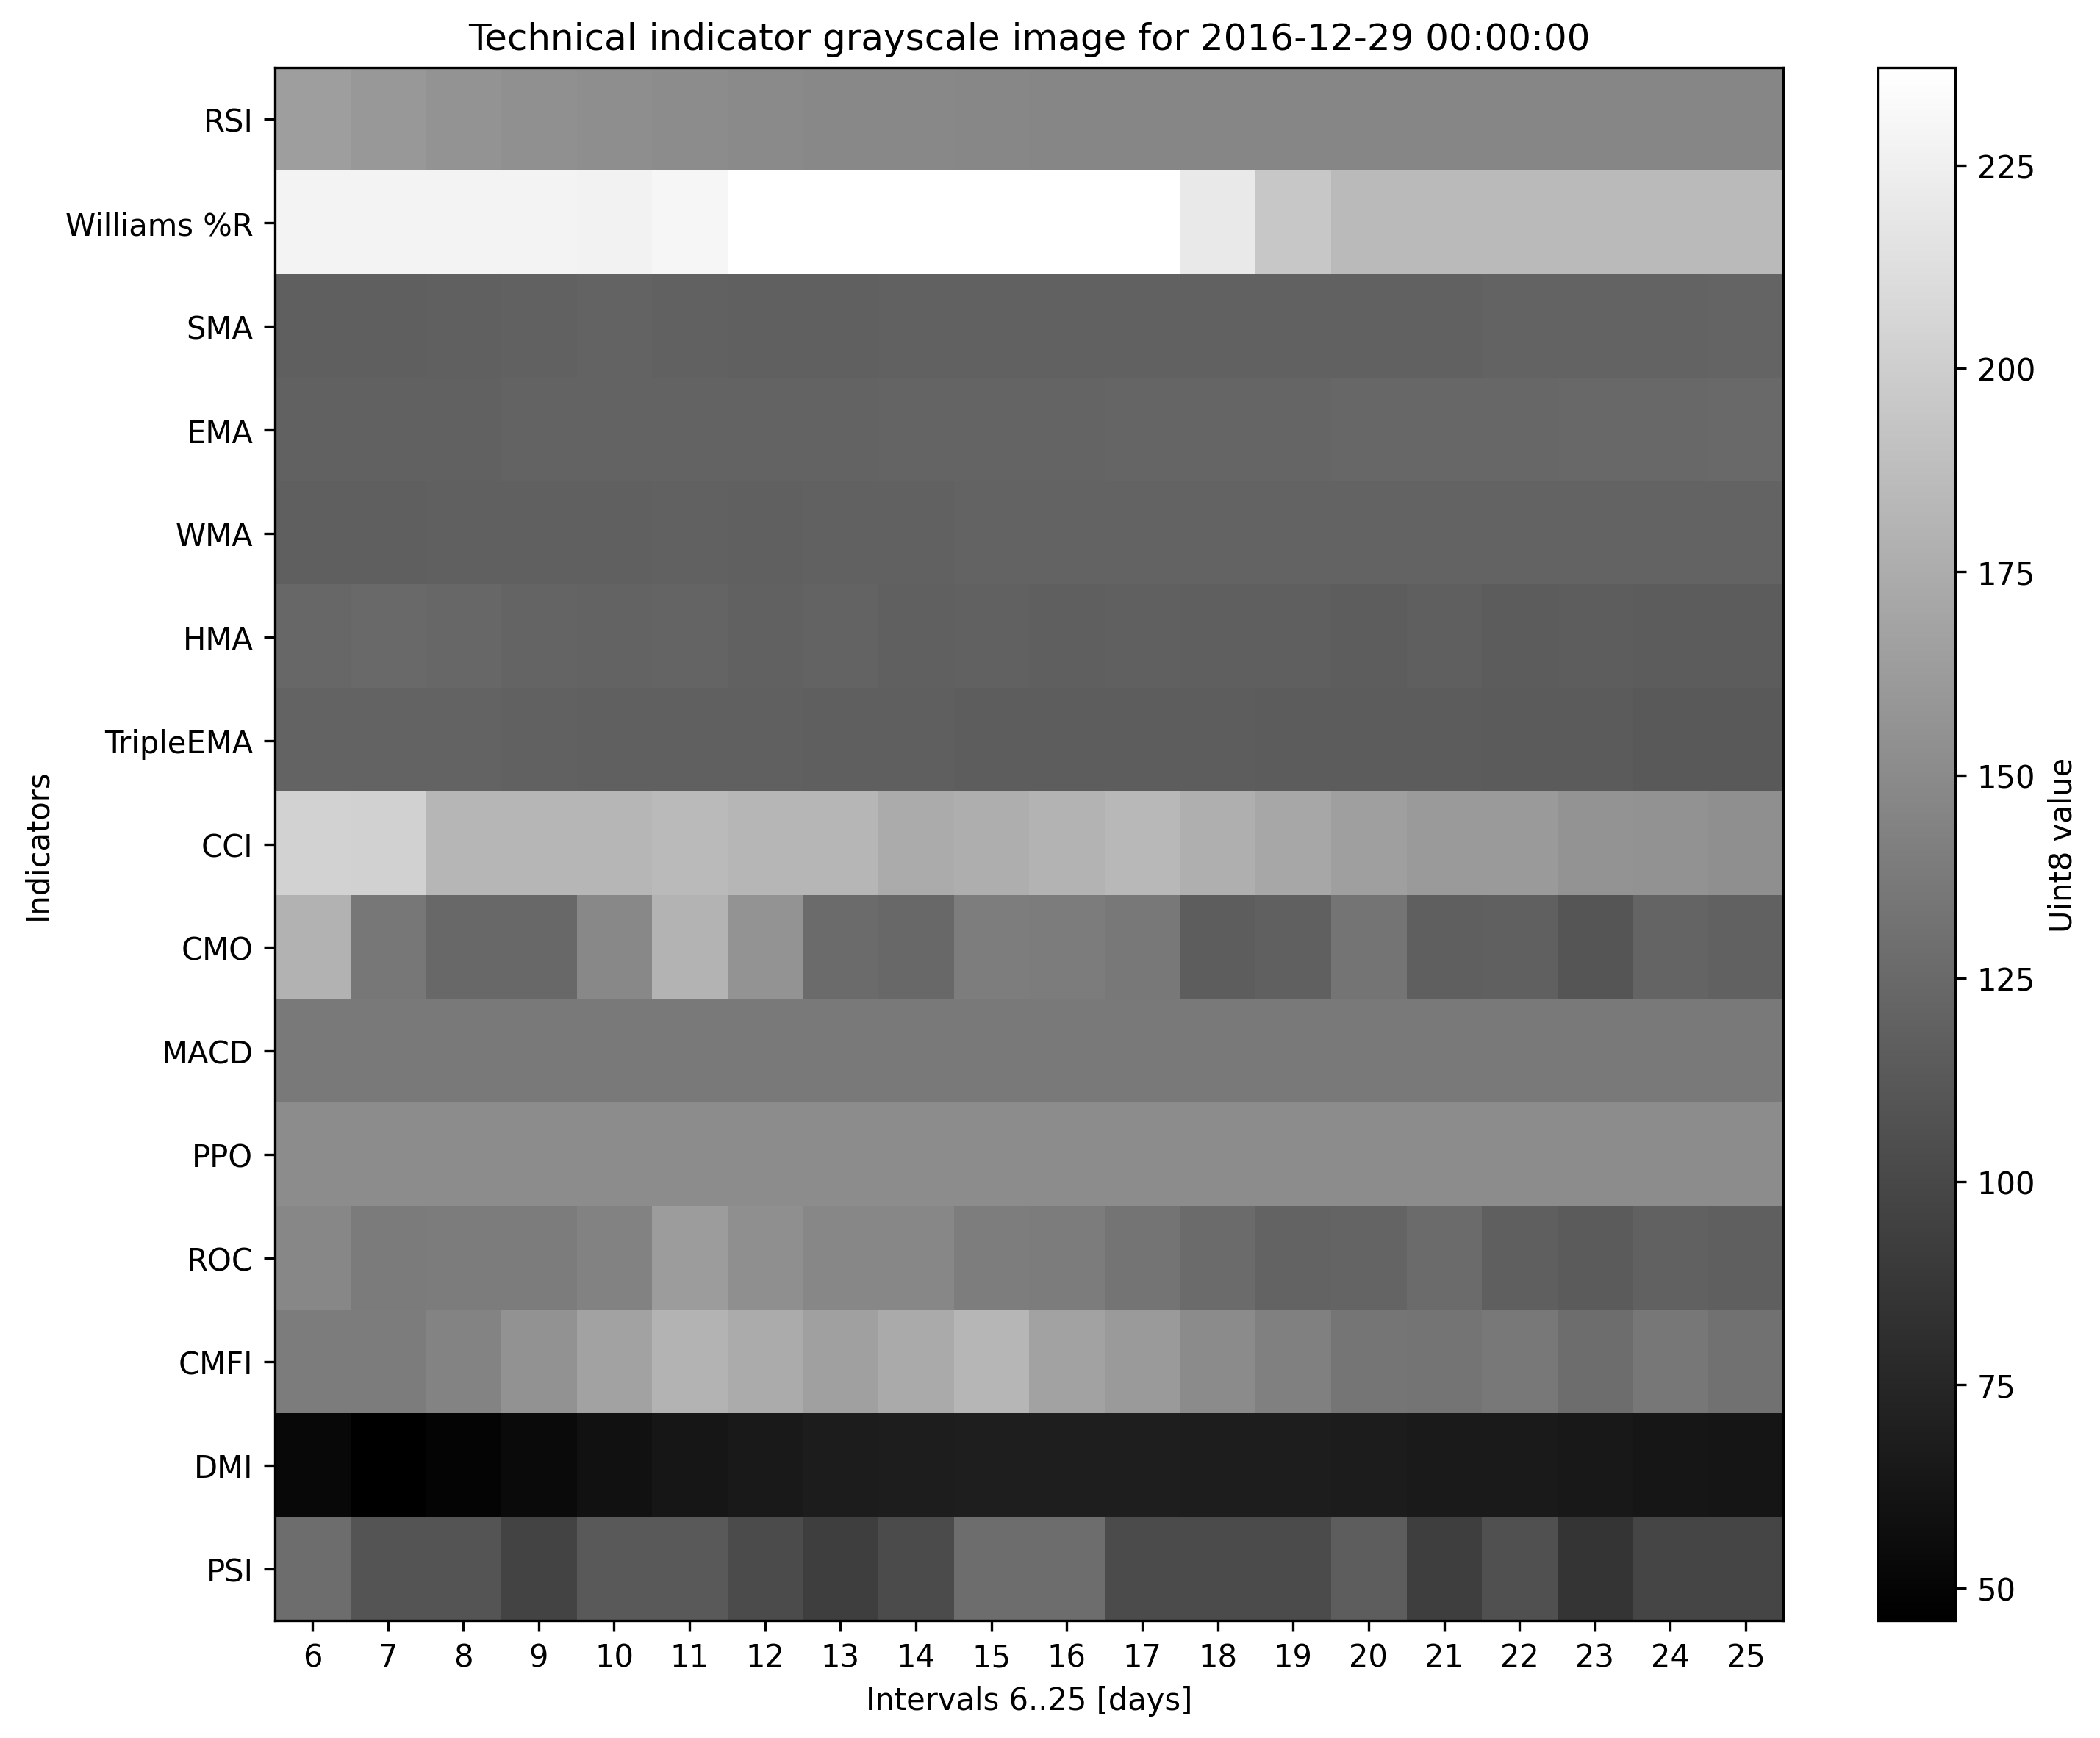
\includegraphics[width=0.6\textwidth]{figures/Technical Indicator.png}
	\caption{Example of a technical–only grayscale image ($15 \times 20$). The vertical axis lists the fifteen technical indicators, and the horizontal axis shows lookback windows from six to twenty–five days.}
	\label{fig:tech_only_image}
\end{figure}

Figure~\ref{fig:tech_macro_image} illustrates the combined representation, where the five macroeconomic rows are appended beneath the technical indicators to form a $20 \times 20$ image.

\begin{figure}[H]
	\centering
	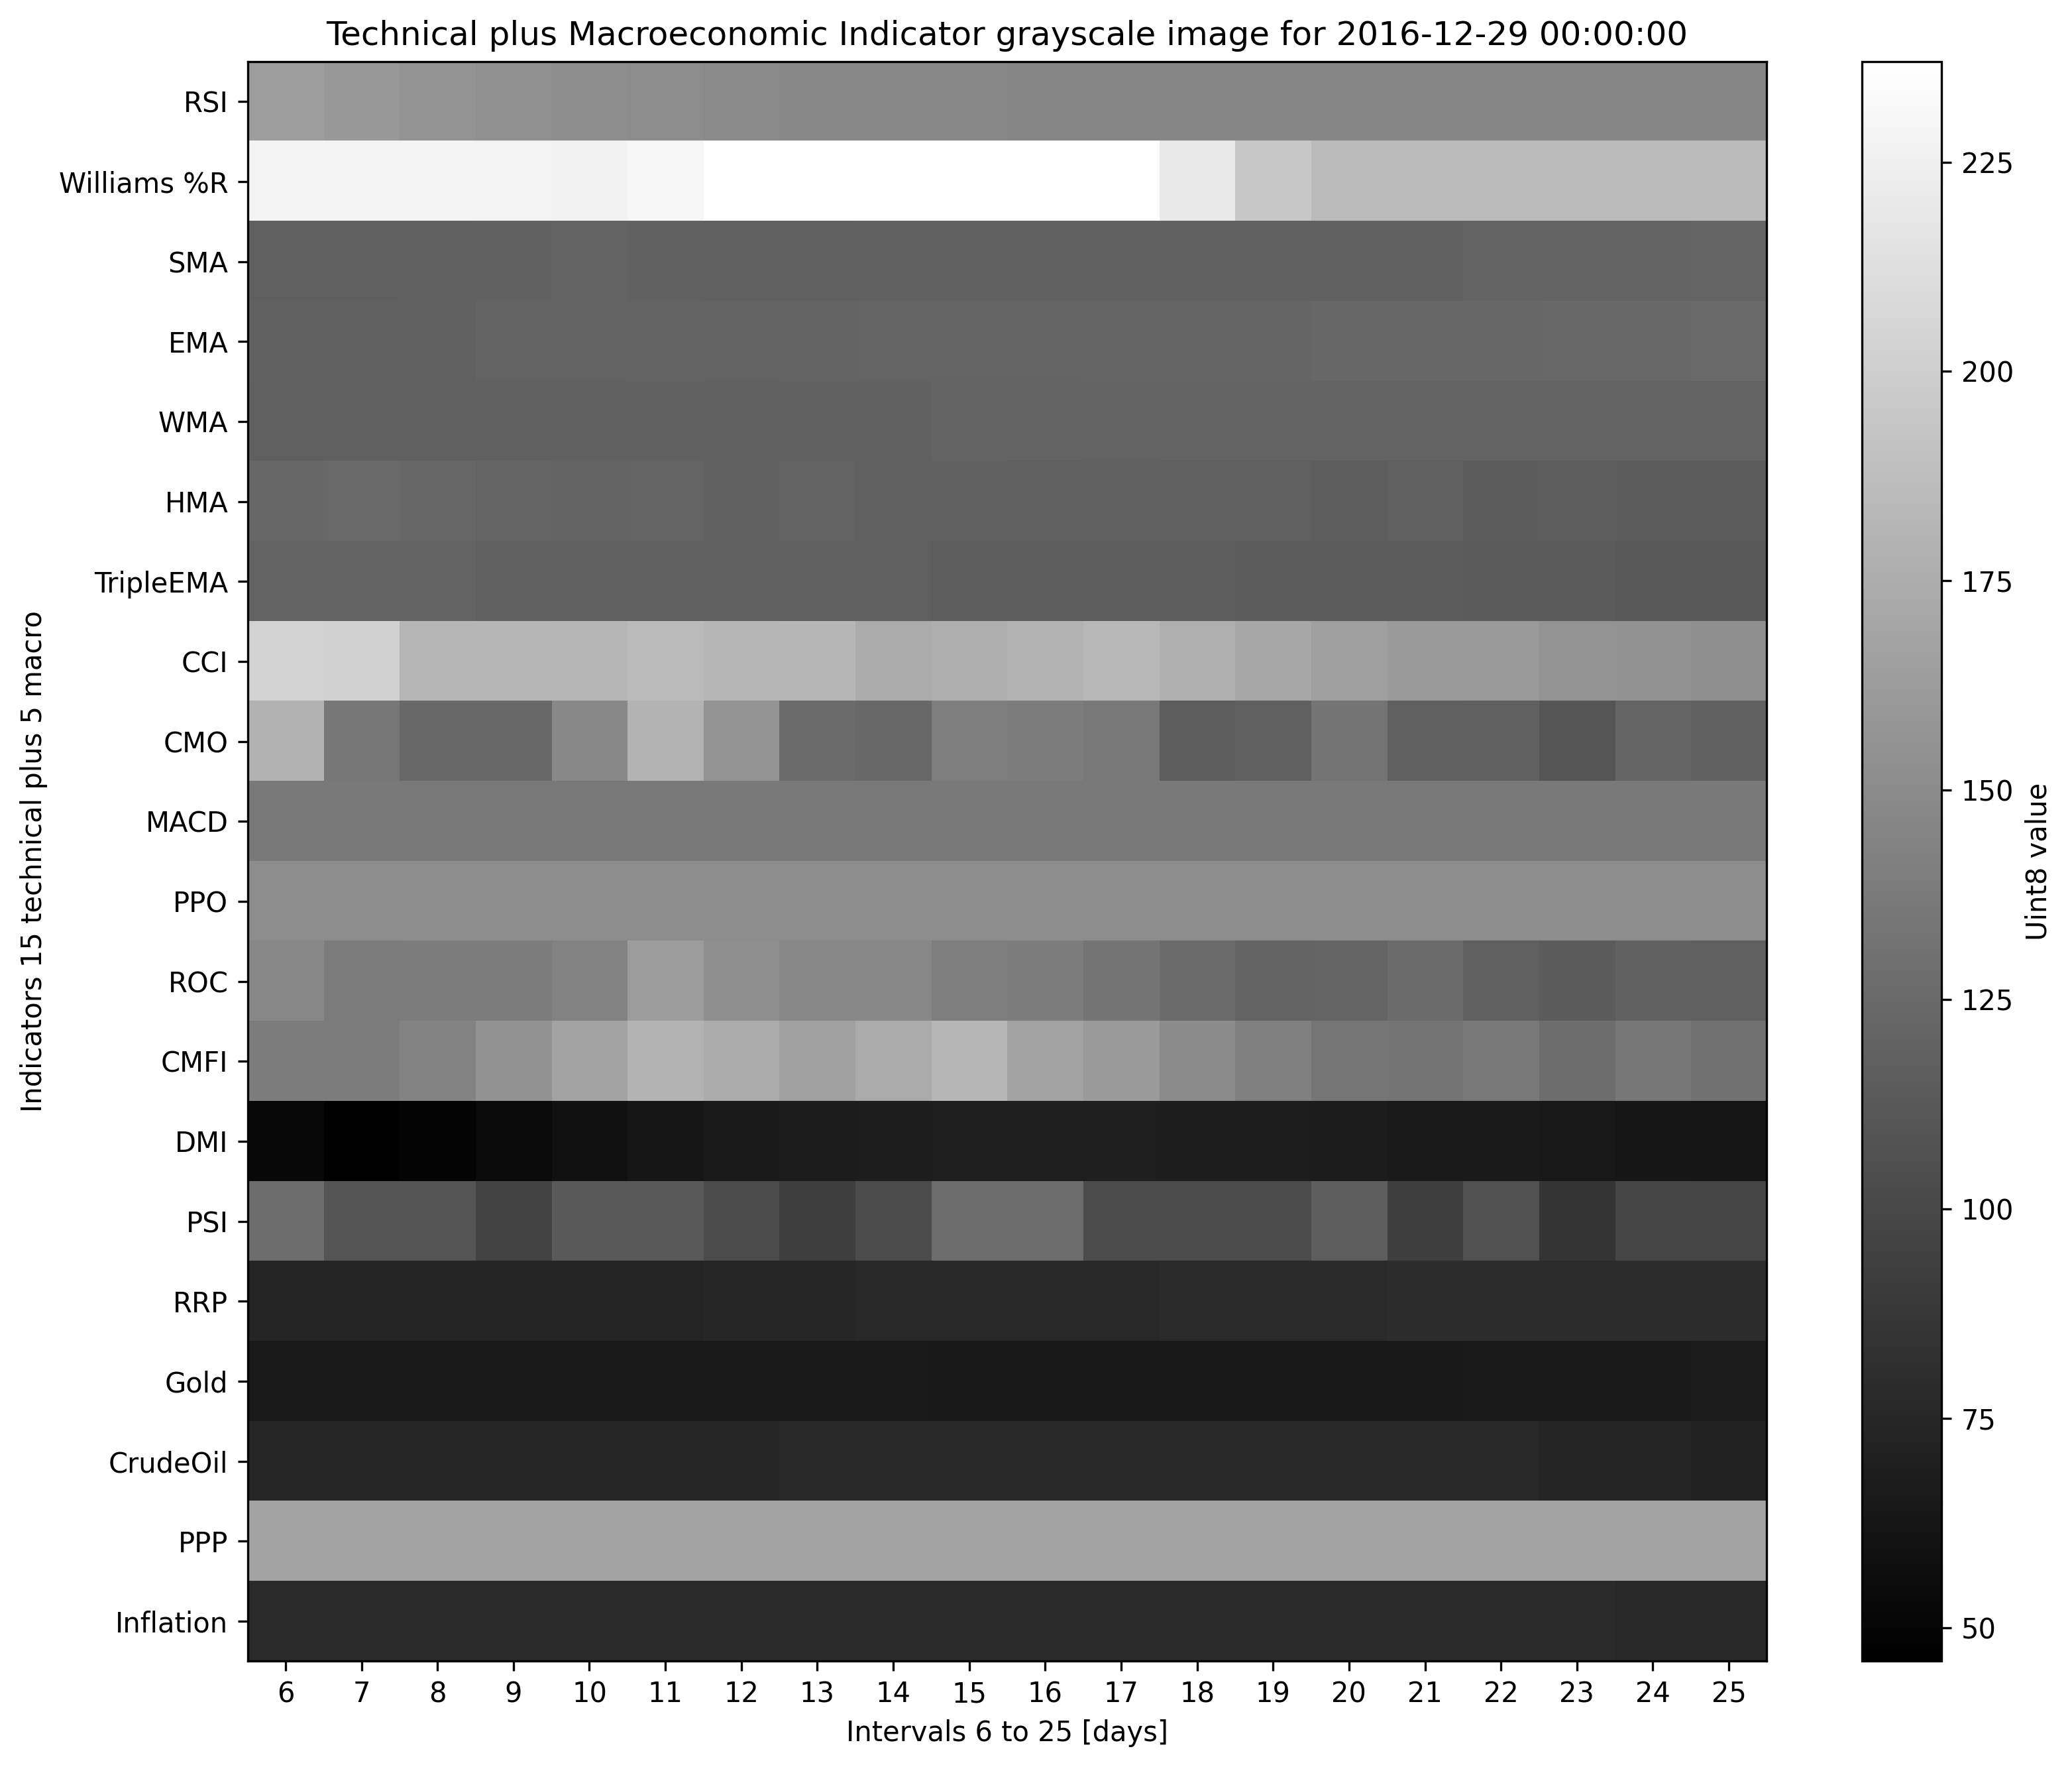
\includegraphics[width=0.6\textwidth]{figures/CombinedTechandMacro.png}
	\caption{Combined technical and macroeconomic grayscale image ($20 \times 20$). Rows 16–20 contain RRP, Gold, CrudeOil, PPP, and Inflation, aligned to the same set of lookback windows.}
	\label{fig:tech_macro_image}
\end{figure}

Overall, these two forms show how the normalized and quantized indicator values are encoded into $15 \times 20$ and $20 \times 20$ grayscale images that serve as inputs to the CNN models.

\subsection{Model Training}
\label{subsec:model-training}

This stage trains two convolutional models under identical settings to allow a fair comparison between the technical only baseline and the combined technical–macroeconomic approach. The baseline model, CNN--TIC, receives a $15 \times 20$ grayscale image that encodes only the technical indicators. The proposed model, CNN--MIC, refers to a Convolutional Neural Network with Macroeconomic-Integrated Channels. It receives a $20 \times 20$ image where the technical indicators and the macroeconomic series are integrated into a single representation.


\begin{figure}[H]
	\centering
	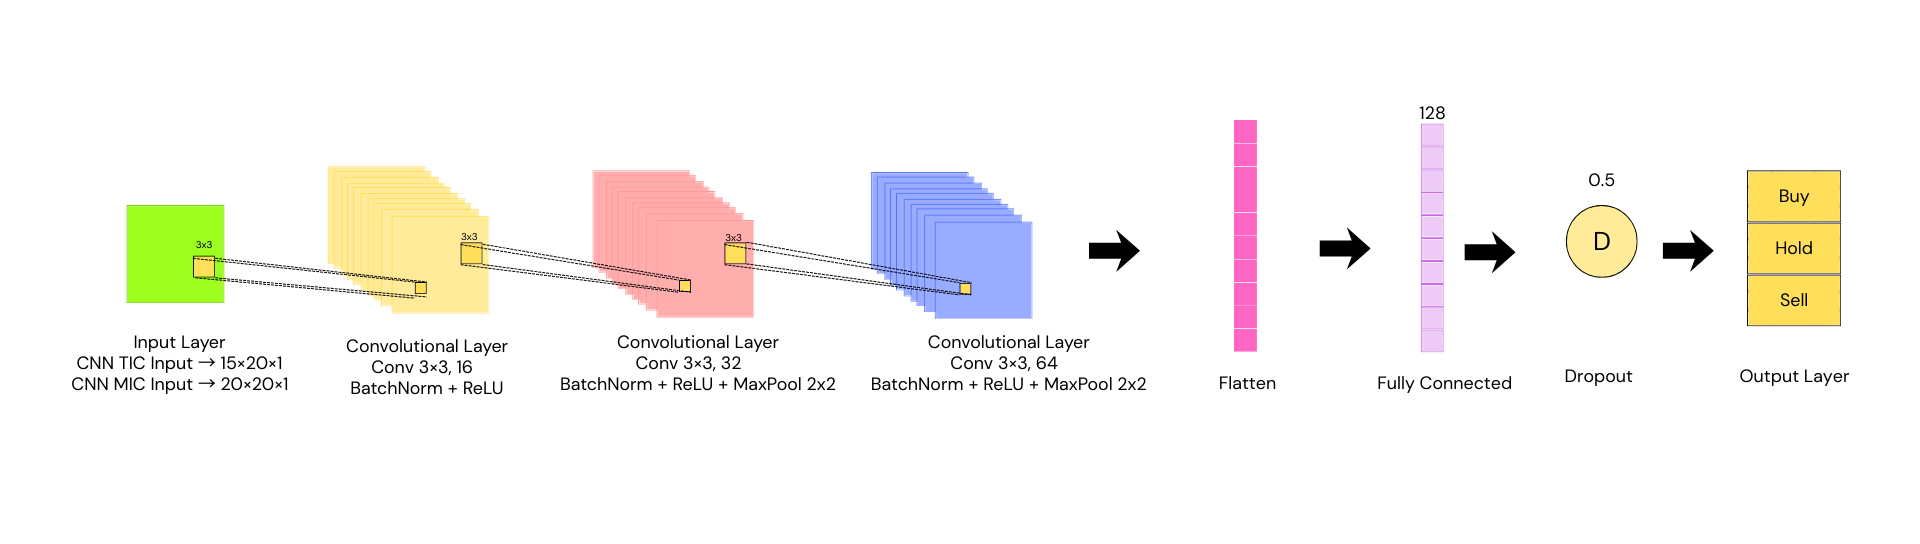
\includegraphics[width=1\textwidth]{figures/CNN_Architecture.png}
	\caption{SmallCNN\_BN architecture used for both CNN--TIC and CNN--MIC. The network applies three convolutional blocks with batch normalization and ReLU, followed by flattening, a fully connected layer with 128 units, dropout, and a three-unit softmax output.}
	\label{fig:smallcnn-architecture}
\end{figure}

\paragraph{Architecture}

The architecture follows the design principles of earlier image-based trading systems such as CNN--TIC, which showed that shallow convolutional structures are effective for indicator-based images. In this study, the input images are much smaller than those used in standard vision applications. The technical only images measure $15 \times 20$, and the combined images measure $20 \times 20$. Because of these constraints, deeper architectures and standard vision backbones are unsuitable.

To address this, a compact model called \textbf{SmallCNN\_BN} was constructed. The model adapts the general ideas demonstrated in prior CNN trading literature but is redesigned to match the spatial layout of the technical and macroeconomic representations. The objective is to provide enough capacity to detect local spatial patterns while controlling the risk of overfitting.

The feature extractor consists of three sequential convolutional blocks:

\begin{itemize}
	\item Block 1: Conv($3 \times 3$, 16 filters), BatchNorm, ReLU.
	\item Block 2: Conv($3 \times 3$, 32 filters), BatchNorm, ReLU, MaxPool($2 \times 2$).
	\item Block 3: Conv($3 \times 3$, 64 filters), BatchNorm, ReLU, MaxPool($2 \times 2$).
\end{itemize}

The output of the convolutional blocks is flattened and passed into a fully connected layer with 128 units and ReLU activation. A dropout layer (probability $0.5$) reduces overfitting. The final linear layer outputs three logits corresponding to the Buy, Hold, and Sell classes, followed by a softmax to produce class probabilities.

\paragraph{Training procedure}

Both models use the same training configuration to isolate the effect of the input representation. Weighted cross entropy is used as the loss function with a label smoothing factor of $0.05$. Class weights are computed from the training split using inverse class frequency to reduce the effect of strong class imbalance in the Buy and Sell categories.

Training uses the AdamW optimizer with a learning rate of $10^{-3}$, weight decay of $10^{-4}$, batch size of $128$, and a cosine annealing learning rate schedule. Each model is trained for $50$ epochs. For every cross-validation fold, the checkpoint with the highest validation macro F1 is retained.

\paragraph{Decision rule}

During inference, the predicted class for day $t$ is obtained by an argmax over the softmax probabilities:

\[
\hat{y}_t = \arg\max_{c \in \{\text{Buy, Hold, Sell}\}} \hat{p}_{t,c}.
\]

The class labels are then mapped into the trading actions used by the financial evaluation procedure described in Algorithm~\ref{alg:financial-evaluation}. This produces a sequence of actionable signals that are passed into the backtesting stage of the framework.



\begin{algorithm}[H]
	\footnotesize
	\caption{FinancialEvaluation}
	\label{alg:financial-evaluation}
	\begin{algorithmic}[1]
		\Procedure{FINANCIALEVALUATION}{}
		\State $balance = 10000$ PHP
		\State $bought\_amount = 0$
		\State $commission = 50$ PHP
		\State $take\_profit = 10\%$
		\State $stop\_loss = 1\%$
		\ForAll{$(price, predicted\_action)$ in $testDataset$}
		\If{$bought\_amount \neq 0$}
		\If{$price > take\_profit\_price$}
		\State $balance = bought\_amount * take\_profit\_price - commission$
		\State $bought\_amount = 0$
		\EndIf
		\If{$price < stop\_loss\_price$}
		\State $balance = bought\_amount * stop\_loss\_price - commission$
		\State $bought\_amount = 0$
		\EndIf
		\EndIf
		\If{$predicted\_action == BUY$ and $balance \neq 0$}
		\State $bought\_amount = (balance - commission) / price$
		\State $balance = 0$
		\State $take\_profit\_price = price * (1.0 + take\_profit / 100)$
		\State $stop\_loss\_price = price * (1.0 - stop\_loss / 100)$
		\EndIf
		\If{$predicted\_action == SELL$ and $bought\_amount \neq 0$}
		\State $balance = bought\_amount * price - commission$
		\State $bought\_amount = 0$
		\EndIf
		\EndFor
		\State \Return $balance$
		\EndProcedure
	\end{algorithmic}
\end{algorithm}

\subsection{Model Evaluation}
\label{subsec:model-eval}

This stage evaluates the models along two dimensions: classification accuracy and trading performance. The first set of metrics measures how well the models predict the Buy, Hold, and Sell classes. The second set measures how these predictions translate into financial outcomes when executed under a fixed trading strategy.

\paragraph{Classification metrics}

Accuracy and macro F1 are used to assess classification performance. These metrics are computed for every fold during cross validation and averaged to obtain a stable estimate of model behavior. After training on the full training pool, the same metrics are computed on the test period to evaluate generalization.


\paragraph{Trading metrics}

To assess economic relevance, the predicted labels are converted into trading actions using the rules defined in Algorithm~\ref{alg:financial-evaluation}. The evaluation uses fixed parameters for both models to ensure a fair comparison. A Buy signal opens a long position on the next market open. A Sell signal closes any existing position. A Hold signal maintains the current position. Each transaction includes a 50-peso commission. The strategy applies a take-profit threshold of 10 percent and a stop-loss threshold of 1 percent relative to the entry price.

\paragraph{Output}

The procedure produces yearly returns, mean annual return, and final equity for the test period. These metrics allow the framework to determine whether improvements in representation lead to measurable gains in trading performance under identical simulation settings.




\section{Initial Experiments and Results}
\label{subsec:initial-results}
This section summarizes the initial experimental results using the SmallCNN\_BN architecture for both the technical only baseline (CNN--TIC) and the proposed technical plus macro model (CNN--MIC). All models are trained on the period 2012 to 2020, evaluated by cross validation on the same period, then tested on the test period 2021 to 2025. The financial performance is finally evaluated using the backtesting procedure in Algorithm~\ref{alg:financial-evaluation}.

\subsection{Cross validation on the training period (2012 to 2020)}

 During model development, a stratified ten-fold cross validation is performed on the training pool, which contains all dates from the start of the dataset until 31 December 2020. For each fold the SmallCNN\_BN model is trained for 50 epochs with class weighted loss, the best checkpoint on validation macro F1 is kept, and the accuracy and macro F1 over the fold validation split are recorded. The mean and standard deviation over the ten folds are reported in Table~\ref{tab:cv-smallcnn-bn}.

\begin{table}[H]
	\centering
	\caption{Cross validation results on 2012 to 2020 using SmallCNN\_BN, ten stratified folds on the training pool.}
	\label{tab:cv-smallcnn-bn}
	\small
	\begin{tabular}{|c|c|c|c|c|}
		\hline
		Model & Mean accuracy & Std accuracy & Mean macro F1 & Std macro F1 \\
		\hline
		CNN--TIC & 0.6819 & 0.0498 & 0.5156 & 0.0264 \\
		\hline
		CNN--MIC & 0.6533 & 0.0253 & 0.4969 & 0.0185 \\
		\hline
	\end{tabular}
\end{table}


The cross validation accuracies suggest that both variants of SmallCNN\_BN reach a moderate level of classification performance on the training period, with CNN--TIC slightly ahead of CNN--MIC in terms of both mean accuracy and mean macro F1 when averaged over years up to 2020. This behaviour is likely related to the strong class imbalance of the Buy and Sell classes and the added difficulty of learning from both technical and macroeconomic channels simultaneously.

\subsection{Test set classification results (2021 to 2025)}

After cross validation, a final SmallCNN\_BN model is retrained on the full training pool (2012 to 2020) then applied to the test period 2021 to 2025. Table~\ref{tab:test-metrics-smallcnn-bn} summarizes the overall test accuracy and macro F1 for the three class classification problem, and Tables~\ref{tab:cm-tech-only} and~\ref{tab:cm-tech-macro} show the corresponding confusion matrices.

\begin{table}[H]
	\centering
	\caption{Test set metrics on 2021 to 2025 using SmallCNN\_BN, overall accuracy and macro F1.}
	\label{tab:test-metrics-smallcnn-bn}
	\small
	\begin{tabular}{|c|c|c|}
		\hline
		Model & Test accuracy & Test macro F1 \\
		\hline
		CNN--TIC & 0.6924 & 0.5243 \\
		\hline
		CNN--MIC & 0.6476 & 0.4926 \\
		\hline
	\end{tabular}
\end{table}


 To better understand the distribution of errors across Buy, Hold, and Sell, the confusion matrices for the test period are reported explicitly. The rows correspond to the true class and the columns to the predicted class, ordered as Sell, Hold, Buy.

\begin{table}[H]
	\centering
	\caption{Confusion matrix on 2021 to 2025 for CNN--TIC, rows: true labels, columns: predictions.}
	\label{tab:cm-tech-only}
	\small
	\begin{tabular}{|c|c|c|c|}
		\hline
		& Predicted Sell & Predicted Hold & Predicted Buy \\
		\hline
		True Sell & 47 & 32 & 0 \\
		\hline
		True Hold & 120 & 676 & 178 \\
		\hline
		True Buy & 0 & 20 & 65 \\
		\hline
	\end{tabular}
\end{table}


\begin{table}[H]
	\centering
	\caption{Confusion matrix on 2021 to 2025 for CNN--MIC, rows: true labels, columns: predictions.}
	\label{tab:cm-tech-macro}
	\small
	\begin{tabular}{|c|c|c|c|}
		\hline
		& Predicted Sell & Predicted Hold & Predicted Buy \\
		\hline
		True Sell & 69 & 10 & 0 \\
		\hline
		True Hold & 224 & 623 & 127 \\
		\hline
		True Buy & 0 & 40 & 45 \\
		\hline
	\end{tabular}
\end{table}


 On the full test period 2021 to 2025, the technical only configuration slightly outperforms the combined technical plus macro configuration in terms of both accuracy and macro F1. The confusion matrices show that both models are dominated by the Hold class, with relatively few Buy and Sell events, and that most of the misclassifications for Buy and Sell tend to be absorbed into Hold. This imbalance is consistent with the turning point labeling scheme, where genuine local minima and maxima are rare compared to non turning points.

\subsection{Financial evaluation on the test period}

To evaluate the economic relevance of the predictions, the trading signals are passed into the FinancialEvaluation procedure in Algorithm~\ref{alg:financial-evaluation}. The backtest starts with an initial capital of 10{,}000 PHP, uses a fixed commission of 50 PHP per trade, a take profit of plus 10 percent relative to the entry price, and a stop loss of minus 1 percent. For each model, the backtest produces a final equity value and yearly returns for 2021 to 2025. Table~\ref{tab:financial-smallcnn-bn} summarizes the initial balance, final equity, mean annual return, and standard deviation of annual returns.

\begin{table}[H]
	\centering
	\caption{Financial evaluation on 2021 to 2025 using FinancialEvaluation, initial capital 10{,}000 PHP, commission 50 PHP, take profit 10 percent, stop loss 1 percent.}
	\label{tab:financial-smallcnn-bn}
	\small
	\setlength{\tabcolsep}{2pt} % a bit tighter columns if needed
	\renewcommand{\arraystretch}{2}
	\resizebox{\textwidth}{!}{%
	\begin{tabular}{|p{2.4cm}|p{3.3cm}|p{3.9cm}|*{12}{c|}}
		\hline
		Model & Initial balance [PHP] & Final equity [PHP] & Mean annual return & Std annual return \\
		\hline
		 CNN--TIC   & 10{,}000 & 17{,}384.65 & 0.1132 & 0.1278 \\
		 \hline
		 CNN--MIC  & 10{,}000 & 21{,}715.91 & 0.1655 & 0.1537 \\
		\hline
	\end{tabular}
}
\end{table}

Although CNN--MIC does not surpass CNN--TIC in pure classification metrics on the test period, it achieves a higher final equity and a higher mean annual return in the backtest. This suggests that the combined technical and macro representation may help the model place Buy and Sell signals in more profitable regions of the price series, even if the overall classification accuracy is slightly lower. At the same time, the larger standard deviation of annual returns for CNN-MIC indicates higher variability in year-to-year performance, which can be discussed further in the risk analysis of the strategy.



\section{Schedule of Activities}

\subsection{Year 1}

\begin{table}[H]
	\centering
	\label{tab:sched_year1}
	\small
	\setlength{\tabcolsep}{3pt}
	\renewcommand{\arraystretch}{1.15}
	\begin{tabular}{|p{2.4cm}|p{3.3cm}|p{3.9cm}|*{12}{c|}}
		\hline
		\multicolumn{1}{|c|}{\footnotesize\textbf{OBJECTIVES}} &
		\multicolumn{1}{c|}{\footnotesize\shortstack{\textbf{TARGET}\\\textbf{ACTIVITIES}}} &
		\multicolumn{1}{c|}{\footnotesize\shortstack{\textbf{TARGET}\\\textbf{ACCOMPLISHMENTS}}} &
		\multicolumn{12}{c|}{\textbf{YEAR 1}} \\
		\hline
		& & &
		\textbf{1} & \textbf{2} & \textbf{3} & \textbf{4} & \textbf{5} & \textbf{6} &
		\textbf{7} & \textbf{8} & \textbf{9} & \textbf{10} & \textbf{11} & \textbf{12} \\
		\hline
		
		Objective 1 &
		To enhance the CNN--TIC framework by expanding its technical indicator image matrix to include macroeconomic variables in a unified visual representation. &
		1. Finalize the list of technical and macroeconomic indicators. \newline 
		2. Prepare Python scripts for data loading, cleaning, and alignment to the trading calendar. 
		\newline 
		3. Produce a prototype generator that outputs technical and combined images for selected stocks. &
		 & & & & & & & &  \cellcolor{gray!50} & \cellcolor{gray!50}& &\\
		\hline
		
		Objective 2 &
		To compare model performance using accuracy, macro F1, and annualized return to see whether macroeconomic indicators provide improvements. &
		1. Define the experimental protocol (data splits and labeling rule). 
		\newline 
		2. Implement the baseline CNN--TIC training code using technical only images. 
		\newline
		3. Obtain initial accuracy and macro F1 results for at least one representative stock. &
		 & & & & & & & & & \cellcolor{gray!50}&\cellcolor{gray!50} &\\
		\hline
		
		Objective 3 &
		To evaluate performance on different stock categories in the PSE and on cryptocurrency data. &
		1. Prepare datasets for blue chip stocks, penny stocks, and at least one cryptocurrency. 
		\newline
		2. Document the preprocessing pipeline for reuse in Year 2 experiments. &
		 & & & & & & & & & &\cellcolor{gray!50} &\cellcolor{gray!50}\\
		\hline
		
	\end{tabular}
\end{table}



\subsection{Year 2}

\begin{table}[H]
	\centering
	\label{tab:sched_year2}
	\small
	\setlength{\tabcolsep}{3pt}
	\renewcommand{\arraystretch}{1.15}
	\begin{tabular}{|p{2.4cm}|p{3.3cm}|p{3.9cm}|*{12}{c|}}
		\hline
		\multicolumn{1}{|c|}{\footnotesize\textbf{OBJECTIVES}} &
		\multicolumn{1}{c|}{\footnotesize\shortstack{\textbf{TARGET}\\\textbf{ACTIVITIES}}} &
		\multicolumn{1}{c|}{\footnotesize\shortstack{\textbf{TARGET}\\\textbf{ACCOMPLISHMENTS}}} &
		\multicolumn{12}{c|}{\textbf{YEAR 2}} \\
		\hline
		& & &
		\textbf{1} & \textbf{2} & \textbf{3} & \textbf{4} & \textbf{5} & \textbf{6} &
		\textbf{7} & \textbf{8} & \textbf{9} & \textbf{10} & \textbf{11} & \textbf{12} \\
		\hline
		
		Objective 1 &
		To train and evaluate the proposed CNN--MIC model that integrates both technical and macroeconomic indicators. &
		1. Complete training runs for CNN--MIC across the prepared datasets. 
		\newline 
		2. Record classification metrics (accuracy and macro F1) for all stocks and categories. &
		\cellcolor{gray!50} & \cellcolor{gray!50} & \cellcolor{gray!50} & & & & & & & & & \\
		\hline
		
		Objective 2 &
		To compare the trading performance of CNN--TIC and CNN--MIC under a unified backtesting framework. &
		1. Implement trading simulation with fixed take profit and stop loss rules. 
		\newline
		2. Compute annualized return, Sharpe ratio, and other trading metrics. 
		\newline
		3. Identify conditions where CNN--MIC improves over CNN--TIC. &
		&\cellcolor{gray!50} & \cellcolor{gray!50} & \cellcolor{gray!50} & & & & & & & & \\
		\hline
		
		Objective 3 &
		To evaluate feature importance and model behavior, interpreting how macroeconomic information contributes to CNN decisions. &
		1. Generate per class confusion matrices and per indicator analyses. 
		2. Summarize how macro rows change predictions across different market conditions. &
		& & \cellcolor{gray!50} & \cellcolor{gray!50} & & & & & & & & \\
		\hline
		
		Objective 4 &
		To document, refine, and finalize the thesis manuscript. &
		1. Draft and revise chapters on methodology, results, and discussion. 
		\newline
		2. Finalize tables, figures, and appendices. 
		\newline
		3. Prepare the final manuscript for submission and final defense. &
		& & \cellcolor{gray!50} & \cellcolor{gray!50} & \cellcolor{gray!50}& & & & & & & \\
		\hline
		
	\end{tabular}
\end{table}

\newpage
\printbibliography

\end{document}